\section{My implementation of the L* and NL*}
While studying the two algorithms, I started to implement them because I thought that it was a good idea to see how they do concretely work.

The programming language I used is \textit{TypeScript}, the typed version of \textit{Javascript}. I decided to use it because I like typed languages and also because, one compiled, \textit{JavaScript} can be run both on browsers and in terminal thanks to \textit{NodeJs} (a good \textit{Javascript} run time environment).

I have started to organize my \textit{GitHub} repository and created these folders:
\begin{itemize}
  \item \textit{pdf\_src} which contains the main papers I studied during my \textit{TER};
  \item \textit{report} with the \LaTeX{} source files to build this report;
  \item \textit{src} containing the \textit{TypeScript} source files;
  \item \textit{public} where I put the public \textit{JavaScript} libraries to render \textit{Automata} (the \textit{d3-graphviz.js} file) and to make operations between \textit{Automata} (the \textit{noam.js} file);
  \item \textit{dist} which is the folder where the \textit{TypeScript} compiler creates the compiled \textit{JavaScript} files;
  \item \textit{statistics} containing the results of my comparisons of performances between \textit{L*} and \textit{NL*};
\end{itemize}

\subsection{About the Teacher}

A major problem that I soon had to overcome was represent the interactions between Learner and Teacher, (see \cref{eq:interactions}). That's why  I did not only have to implement the Learner, but also the Teacher.

As said in the Introduction, a \textit{Teacher} is an entity knowing the language and answering to membership and equivalence queries. It is quite easy to see how a membership query can be answered: the Teacher can test if the received word belongs to its language.

However it is less evident how the \textit{Teacher} could verify if a conjecture is valid or if not to send the counter-example.

\begin{definition}
  In \cite{LPaper}, a \textit{Teacher} providing every time a counter-example of shortest length is called \textit{Minimal Adequate Teacher}.
\end{definition}

Following this idea, I have decided to implement this king of Teacher because, since the complexity of the algorithms also depends on the length of the counter-examples, it would have been more interesting to reduce as much as possible the value of $m$ obtaining therefore a complexity of $O(n^3)$.

From this moment on, I will consider a Teacher to be the \textit{Minimal Adequate Teacher}.

When the \textit{Learner} sends the conjecture $\A$, the \textit{Teacher} has to perform the symmetrical difference between $\U$ and $\LA$ to find the counter-example of shortest length. This operation can be made in the following way:

\begin{algorithm}
  \caption{Shortest counter-example in $U \Delta \LA$}
  $\A_1 \gets \LA \cap \overline{\U}$\;
  $\A_2 \gets \overline{\LA} \cap \U$\;
  $w_1 \gets \text{ the shortest word accepted by } \A_1$\;
  $w_2 \gets \text{ the shortest word accepted by } \A_2$\;
  \Return shortest($w_1, w_2$)\;
\end{algorithm}

The first two lines of this code are in fact those who are the most expensive in time complexity in my project.

But first, before executing this algorithm, I had to find a way to correctly represents the Learner's conjecture and the Teacher's language to operate in a second moment the intersection and the complementation.

\subsection{Learner's Conjecture and Teacher's Language representation}

The best way I found to represent the Teacher's Language was to think about the way the Learner's conjecture is naturally given by the two algorithms: an automaton. That's why I decided to also represent the Teacher's Language on the form of an automaton.

Therefore, I implemented the Automaton class which has some key attributes to identify the main characteristics of an automaton but before, after some reflection, I also decided to create a \textit{State} class representing the states of the \textit{Automaton} where I added the information of successors (and predecessors) as attributes attached to the instancies of the class.

Finally I had:


\begin{lstlisting}[caption=State class]
class State {
  isAccepting: boolean;
  isInitial: boolean;
  alphabet: string[];
  outTransitions: Map<string, State[]>;
  inTransitions: Map<string, State[]>;
  successors: Set<State>;
  predecessor: Set<State>;
  name: string;

  ... 

  addTransition(symbol: string, state: State): void;
  getSuccessor(symbol: string): State;
  getPredecessor(symbol: string): State;
}
\end{lstlisting}

This implementation exploit a lot the \textit{Map} data-structure which is a fast way in \textit{JavaScript} to get a value from a given key. Since the Automaton can be not deterministic \textit{outTransition} associates a list of \textit{State}s to every symbol of the alphabet.

Moreover a \textit{State} ``knows'' if it is initial an accepting.

Now I had the representation of a state and the class Automaton could be represented as:

\begin{lstlisting}[caption = Automaton class]
class Automaton {
  states: Map<string, State>;
  initialStates: State[];
  acceptingStates: State[];
  allStates: State[];
  alphabet: string[];

  ... 

  accept_word_nfa(word: string): boolean;
  minimize(): Automaton;
\end{lstlisting}

We can see that all the fundamental element of the automaton are represented, there is the list of states, followed by the list of accepting and initial states. The alphabet is a list of string.

The transition function $\delta$ is a bit more difficult to see. But it can deduced thanks the \textit{outTransition} attributes of a \textit{State}.

After the \textit{State} and the \textit{Automaton} class I needed a way to make the union, intersection, complementation on two automata.

To do that I used the \textit{noam.js} library which contains some these useful method. The next thing that I had to do was therefore to create an \textit{Adapter} to transform my representation of an \textit{Automaton} to his representation and vice-versa.

Having these ingredients, $\LA \cap \overline{\U}$ and $\overline{\LA} \cap \U$ could be easily calculated. I only want to point out that the complementation of an automaton takes linear time if the automaton is deterministic we modify the final states in $F' = \Q - F$ but if the automaton is not deterministic, that's the case for the \textit{NL*} algorithm, the only way we know to make the complementation is to determinize before the automaton which is a computationally difficult task.

\subsection{Teacher shortest counter-example}
To find the \textit{shortest} counter-example, in a first time I minimize the automaton with the Hopcroft's algorithm implemented in the \textit{Automaton} class. This algorithm has a complexity $O(n \log n)$. Then, I perform a \textit{BFS} search from the initial states\footnote{The initial states can be multiple in the NL*, that's why a use the plural.} to find the word of shortest length accepted by the Automaton.

I want to underline that if two automata, $\A_1$ and $\A_2$ are equivalent then $\A_1 \Delta \A_2$ gives a new automaton $\A_3$ which recognizes the emptyset $\varnothing$. If $\mathcal{\A}_1 \neq \mathcal{\A}_2$ then it exists at least a word which is accepted by $\A_1$ and not by $\A_2$ or vice-versa. When I launch the \textit{BFS} in $\A_3$, if no word is found, I return $\varnothing$ (I symbolize it with a string of length 0 in \textit{JavaScript}) or the counter-example in the other case.

\subsection{The Observation Table}
The Observation Table is implemented like this.

\begin{lstlisting}[caption = Observation\_table class]
  class Observation_table {
    private rows: string[];
    private columns: string[];
    private matrix: boolean[][];
  
    add_column(column_name: string): void;
    set_value(row_name: string, column_name: string, bool: boolean): void;
    add_row(row_name: string): void;
    get_value(row_name: string, column_name: string): boolean;
    get_row(row_name: string): boolean[];
  }
  \end{lstlisting}

It is a matrix of boolean with two dimensions indexed by rows (the $S$ and $SA$ sets) and columns (the $E$ set).

If the Learner wants to set to $b$ to value of the cell corresponding to the concatenation of the words $\omega_1$ and $\omega_2$ then
\[matrix[rows.indexOf(\omega_1)][columns.indexOf(\omega_2)] = b;\]

A little precision: the \textit{matrix} is initialized in this way $matrix = [[]]$. When we add an element $e$ at position $(x, y)$ with $x > len(matrix)$ and $y > len(matrix[0])$, $JavaScript$ won't raise the error \textit{OutOfBound} such as other programming languages, but instead it will automatically allocated the needed memory and affect the $matrix[x][y]$ to $e$.

\subsection{The Learners implementation}

In this section I want to talk about how I have been able to represent the two Learners.

First of all, I realized that L* and NL* have in common some definitions. That's why I created a common abstract class which implements the shared methods and attributes of the algorithms.

\begin{lstlisting}[caption = LearnerBase class]
abstract class LearnerBase {
  alphabet: string[];
  S: string[];
  E: string[];
  observation_table: ObservationTable;
  SA: string[];
  teacher: Teacher;

  ...

  update_observation_table(key: string, value: string): void;
  make_member(pref: string, suff: string): string;
  make_equiv(a: Automaton): string;
  add_elt_in_S(new_elt: string): void;
  add_elt_in_E(new_elt: string): void;
  move_from_SA_to_S(elt: string): void;

  abstract table_to_update_after_equiv(answer: string): void;
  abstract make_automaton(): Automaton;
  abstract is_close(): string | undefined;
  abstract is_consistent(): string[] | undefined;
}
\end{lstlisting}

The two methods \textit{make\_member} and \textit{make\_equiv} reproduce the interaction with the Teacher. In the two cases the Learner returns a string that is:

\begin{itemize}
  \item ``1'' or ``0'' for membership queries, if the word is accepted or not by the Teacher\footnote{In Javascript there does not exist the type \textit{char}};
  \item a word $\omega$ which represents the counter-example. If $len(\omega) = 0$ then the Learner has understood the language.
\end{itemize}

\textit{add\_elt\_in\_S} and \textit{add\_elt\_in\_E} respectively modify the content of the observation table while adding respectively a row to $S$ as well as all of its prefixes or a column with all its suffixes.

The method \textit{move\_from\_SA\_to\_S} has the same behavior as the \textit{add\_elt\_in\_S} plus it removes the the row moved from SA.

We can see that the abstract methods [Line 20 to 23] correspond to the closedness and consistence properties and to the automaton creation. I also want to underline the \textit{table\_to\_update\_after\_equiv} which modifies the set $S$ if the Learner is L*, the set $E$ otherwise. Both L* and NL* start have a dedicated class extending the \textit{LearnerBase} class.

The NL* algorithm has in addition the \textit{prime\_lines} attribute storing the list of prime rows. It is constantly updated when the \textit{Observation Table} is modified thanks to some useful methods:

\begin{lstlisting}
class NL_start extends LearnerBase {
  prime_rows: string[];

  ... 

  is_prime(row_key: string): boolean;
  row_union(row1: string, row2: string): string;
  is_covered(row1: string, row2: string): boolean;
  check_prime_lines(): void;
}
\end{lstlisting}

These methods are implemented intuitively following the definition explained in \cref{def:row-covering} and \cref{def:row-union}.

\subsection{About the HTML implementation}

All these classes are meant to implement the essential bricks to make the learning algorithms work. However I wanted to display these interactions graphically via the \textit{HTML} language.

To do so, I have created some dedicated classes to manage the web page and display the observation table, the construction of the automata together with the message linked to the closedness and consistence properties.

I have spent some time to find the good library for displaying the Automata. It was not as easy as I thought, at first I have found the \textit{Mermaid} library. The automata displayed were nice, but when they started to have a huge number of state and transitions the drawing started to become less intelligible.

After some further research, I found a way to represent \textit{Dot} files with the \textit{Graphviz} library, which I personally prefer.

\begin{figure}[!htb]
  \centering
  \begin{subfigure}[b]{0.3\textwidth}
    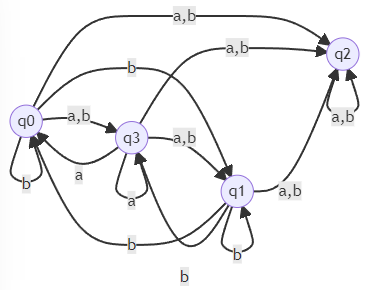
\includegraphics[width=\textwidth]{img/aut_mermaid.png}
    \caption{Automaton in Mermaid}
  \end{subfigure}
  \begin{subfigure}[b]{0.3\textwidth}
    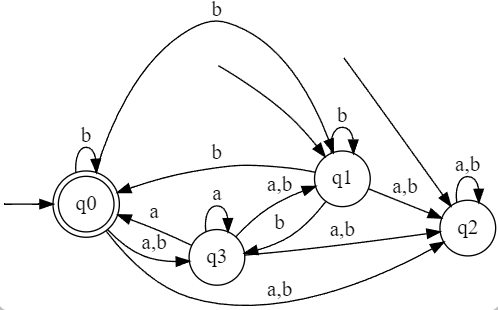
\includegraphics[width=\textwidth]{img/aut_graphviz.png}
    \caption{Automaton with Graphviz}
    \label{fig:graphviz-aut}
  \end{subfigure}
  \caption{Mermaid vs Graphviz}
  \label{fig:mermaidGraphviz}
\end{figure}


In \cref{fig:mermaidGraphviz} we see an example of the two automata representation. The initial and final states are not clearly indicated in the \textit{Mermaid} plot and that the transitions are less clear to understand.

Once I have finished to implement all of this, I have been able to publish my \textit{HTML} page at the url \url{https://fissored.github.io/TER-M1-S2/}.

This page allows you to choose both to run the \textit{L*} and the \textit{NL*} algorithms. Some preloaded Teachers are proposed, but it is also possible to create a custom Teacher by entering a \textit{Regular Expression}.

The regular expression should be encoded with the following grammar:
\[ R = symbol \mid R + R \mid RR \mid R^* \mid(R) \]
The alphabet is composed by every alpha-numeric character and the empty string $\E$ is encoded with $\$$.

\begin{example}
  \[(a + b)+\$+ab^*+(ab)^*\] indicates the language containing $\{\E,a, b,  ab, abb, abbb\dots, ab, abab, ababab\dots\}$.
\end{example}

Once the Teacher created, the user can run step by step or the entire algorithm and every phase of the execution will be displayed.

In the \textit{HTML} page, the \textit{Message} section contains information about the \textit{closedness} and the \textit{consistence} of the $O.T$. Once these two properties are satisfied, the automaton corresponding to the conjecture is displayed (an example is given in \cref{fig:graphviz-aut}).

When an automaton is displayed, you are able to enter a word in the corresponding input section and test if it is accepted or not by the language recognized by the automaton. It can be useful for example to see immediately if the counter-example\footnotetext{The counter-example is also written in the \textit{Message} section.} proposed by the Teacher is accepted or not by the automaton.

The history of the operations made by the \textit{Learner} is saved in memory and can be re-viewed by clicking on the arrows on the side of the screen.